%project-proposal.tex
\documentclass{article}
\usepackage[letterpaper, margin=1.5in]{geometry}
\usepackage{booktabs}
\usepackage{listings}
\usepackage{makecell}
\usepackage{graphicx}

\graphicspath{ {images/} }

\begin{document}


\title{An Experiment of Adversarial Exmaples Crafting and Adversarial Training on Various Datasets}
\author{Jian Li \\ charlee.li@mail.utoroton.ca \and Mingyue Yang \\ myshirley.yang@mail.utoroton.ca}
\maketitle

\begin{abstract}
In this paper, we exercised adversarial example crafting and adversarial training on various datasets and evaluated the performances of crafting and adversarial training.
\end{abstract}

\section{Introduction}

Goodfellow et\ al. and Papernot et.\ al. introduced several algorithms of crafting \emph{adversarial examples}.
These algorithms include \emph{Fast Gradient Sign Method}\cite{goodfellow2015} and \emph{Saliency Map Method}\cite{papernot2015}.
We exercised these two adversarial crafting methods on several datasets and trying to find out the relationship between the datasets and the performance of the algorithm.

We constructed several CNNs with TensorFlow\cite{tensorflow} to recognize several datasets.
Then we modified the CNN model to apply adversarial algorithms (implemented by CleverHans\cite{cleverhans}).
We generated adversarial examples with both algorithms and evaluated their success rate from both misclassification and targeted attack perspectives.
Then we retrained the model with adversarial training, and regenerated adversarial examples to evaluate the performance of the adversarial training.

Due to limited time frame, we were not able to experiment adversarial training with Saliency Map method.

\section{Datasets}

We crafted adversarial examples using different settings on CGTSRB10, CIFAR10, FMNIST, MNISTBG datasets. 

CGTSRB10 is a subset of the original GTSRB\cite{gtsrb} dataset. GTSRB is an image collection consisting of 43 traffic signs. 
These images are captured from real-life videos so that every traffic sign has a serial of images with different resolutions.
For experiment purpuse, we handpicked 10 classes from GTSRB, then cropped the images to the exact frame of the traffic signs
using the annotation data given in the dataset, and resized the images to 32$\times$32 pixels. This dataset is used in RGB mode (colour images).

CIFAR10\cite{cifar10} is an image collection of objects. It contains 60000 32$\times$32 colour images in 10 classes.

FMNIST(Fashion MNIST)\cite{fmnist} is a MNIST-like fashion product dataset. It consists of a training set of 60000 examples and a test set of 10000 examples. Each example is a 28$\times$28 grayscale image, associated with a label from 10 classes. This dataset has exact attribute as MNIST dataset\cite{mnist}, with the images are replaced with fashion objects such as shirts, skirts and shoes.

MNISTBG(MNIST with background)\cite{mnistbg} is a patched version of MNIST dataset. Each MNIST example is attached with a background image extracted randomly from a set of 20 images downloaded from the Internet.

As a comparasion, we did the same experiment on the original MNIST dataset.

\section{CNN Model}

We trained a convolutional neural network model for each dataset.
The architecture and test accuracy of each CNN is described in Table~\ref{tab:cnnarch}.

These CNNs are implemented with TensorFlow\cite{tensorflow}.

\subsection{Experience}

Initially we implemented the CNN model with the \lstinline{Estimator} class to simplify the training and testing process.
However later we found that \lstinline{Estimator} heavily capsulated the model and could not provide enough support for adversarial examples crafting.
Since both fast gradient sign method and saliency map method are whitebox attacks, they require the model to be able to produce
predictions for any given input tensor. Eventually we crafted the model with the following form:

\begin{lstlisting}
class CNNModel:
    def make_model(self, x):
        # construct layers based on input x
        ...
        return output_tensor
\end{lstlisting}

\begin{table}
\centering
\begin{tabular}{llllll}
    \toprule
    Layer & CGTSRB10 & CIFAR10 & FMNIST & MNISTBG & MNIST \\
    \midrule
    0, input &
        32$\times$32$\times$3 &
        32$\times$32$\times$3 &
        28$\times$28$\times$1 &
        28$\times$28$\times$1 &
        28$\times$28$\times$1 \\
    \midrule

    1, cnv & 
        \makecell{knl=5$\times$5 \\ cnv=32$\times$32} & 
        \makecell{knl=3$\times$3 \\ cnv=48$\times$48} &
        \makecell{knl=5$\times$5 \\ cnv=32$\times$32} &
        \makecell{knl=5$\times$5 \\ cnv=32$\times$32} &
        \makecell{knl=5$\times$5 \\ cnv=32$\times$32} \\
    \midrule
    2, pooling &
        2$\times$2 &
        2$\times$2 &
        2$\times$2 &
        2$\times$2 &
        2$\times$2 \\
    \midrule

    3, cnv & 
       \makecell{knl=5$\times$5 \\ cnv=64$\times$64} & 
       \makecell{knl=3$\times$3 \\ cnv=96$\times$96} &
       \makecell{knl=5$\times$5 \\ cnv=64$\times$64} &
       \makecell{knl=5$\times$5 \\ cnv=64$\times$64} &
       \makecell{knl=5$\times$5 \\ cnv=64$\times$64} \\
    \midrule

    4, pooling &
        2$\times$2 &
        2$\times$2 &
        2$\times$2 &
        2$\times$2 &
        2$\times$2 \\
    \midrule

    5, cnv & 
       \makecell{knl=5$\times$5 \\ cnv=128$\times$128} & 
       \makecell{knl=3$\times$3 \\ cnv=192$\times$192} &
       - &
       - &
       - \\
    \midrule

    6, pooling &
        2$\times$2 &
        2$\times$2 &
        - &
        - &
        - \\
    \midrule
    
    7, dense &
        512 &
        512 &
        1024 &
        1024 &
        1024 \\
    \midrule

    8, dense &
        - &
        256 &
        - &
        - &
        - \\
    \midrule

    9, dense &
        10 &
        10 &
        10 &
        10 &
        10 \\

    \midrule

    test accuracy &
        97\% &
        68\% &
        92\% &
        92\% &
        99\% \\

    \bottomrule
\end{tabular}
\caption{\label{tab:cnnarch} CNN models architecture}
\end{table}


\section{Adversarial Examples Crafting}

We used the implmenetation of fast gradient sign method and saliency map method from the CleverHans\cite{cleverhans}.

\subsection{Fast Gradient Sign Method}

For fast gradient sign method, we used 5000 examples from the test set of each dataset (except for CGTSRB10 which has only 3360 test examples) and generated adversarial examples with \(\epsilon=0.1~0.6\).

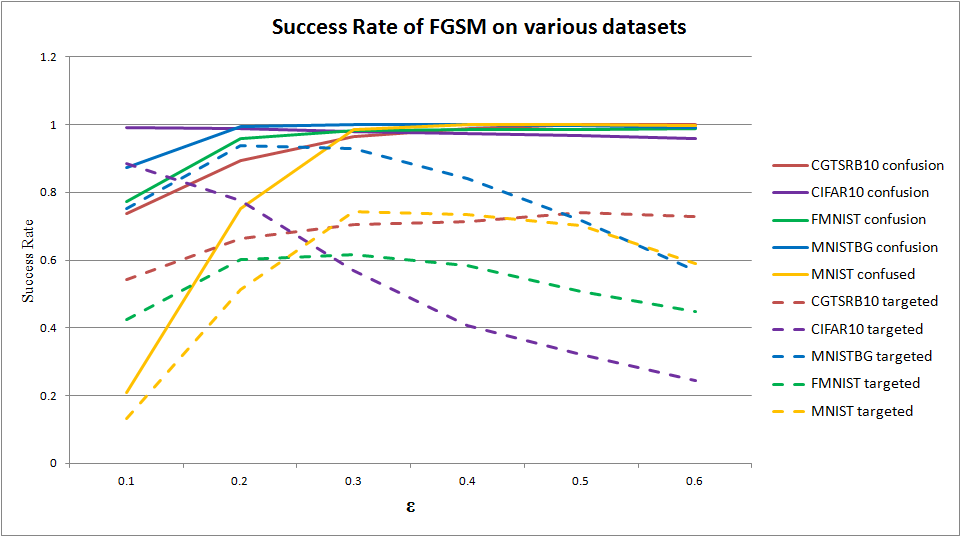
\includegraphics[scale=0.45]{fgsm}


\subsection{Saliency Map Method}

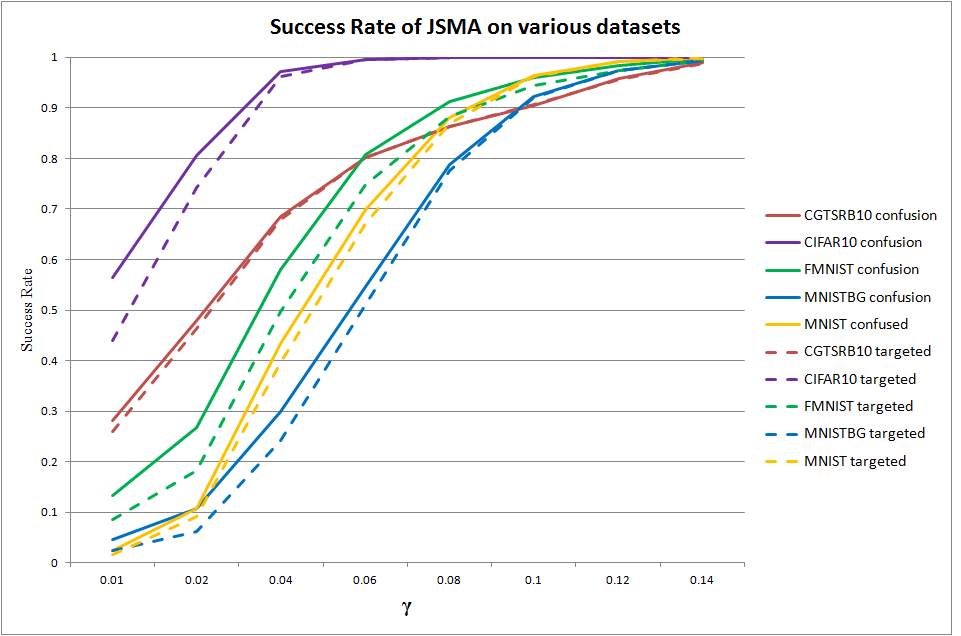
\includegraphics[scale=0.45]{jsma}

\section{Adversarial Training}


\section{Discussion}


\section{Conclusion}


\begin{thebibliography}{9}
\raggedright
\bibitem{goodfellow2015}
    Goodfellow, Ian J et\ al.,
    \emph{Explaining and Harnessing Adversarial Examples},	
    arXiv:1412.6572v3,
    3/2015

\bibitem{papernot2015}
    Nicolas Papernot et.\ al.,
    \emph{The Limitations of Deep Learning in Adversarial Settings},
    arXiv 1511.07528v1,
    11/2015

\bibitem{blackbox2017}
    Nicolas Papernot et.\ al.,
    \emph{Practical Black-Box Attacks against Machine Learning}.
    ASIA CCS '17,
    2017.

\bibitem{cifar10}
    \emph{The CIFAR-10 dataset},
    https://www.cs.toronto.edu/~kriz/cifar.html

\bibitem{gtsrb}
    \emph{German Traffic Sign Recognition Benchmark}.
    http://benchmark.ini.rub.de/?section=gtsrb\&subsection=dataset

\bibitem{fmnist}
    \emph{Fashion MNIST},
    https://github.com/zalandoresearch/fashion-mnist

\bibitem{mnistbg}
    \emph{MNIST with Background},
    http://www.iro.umontreal.ca/~lisa/twiki/bin/view.cgi/Public/MnistVariations

\bibitem{mnist}
    \emph{MNIST},
    http://yann.lecun.com/exdb/mnist/

\bibitem{cleverhans}
    \emph{CleverHans},
    https://github.com/tensorflow/cleverhans

\bibitem{tensorflow}
    \emph{TensorFlow},
    http://tensorflow.org/

\end{thebibliography}


\end{document}
